\subsection{Package \lstinline!cryptocast.comm!}
This package provides functionality related to communication between the different layers
 of the network protocol and to the communication between the server and clients. This includes
 the management of file and socket streams and abstractions of the multi-client unidirectional
 streams that represent the core of this project.
 Useful abstractions for layered protocols are also included.

\noindent\begin{minipage}[t]{5cm}
\vspace{0.3em}
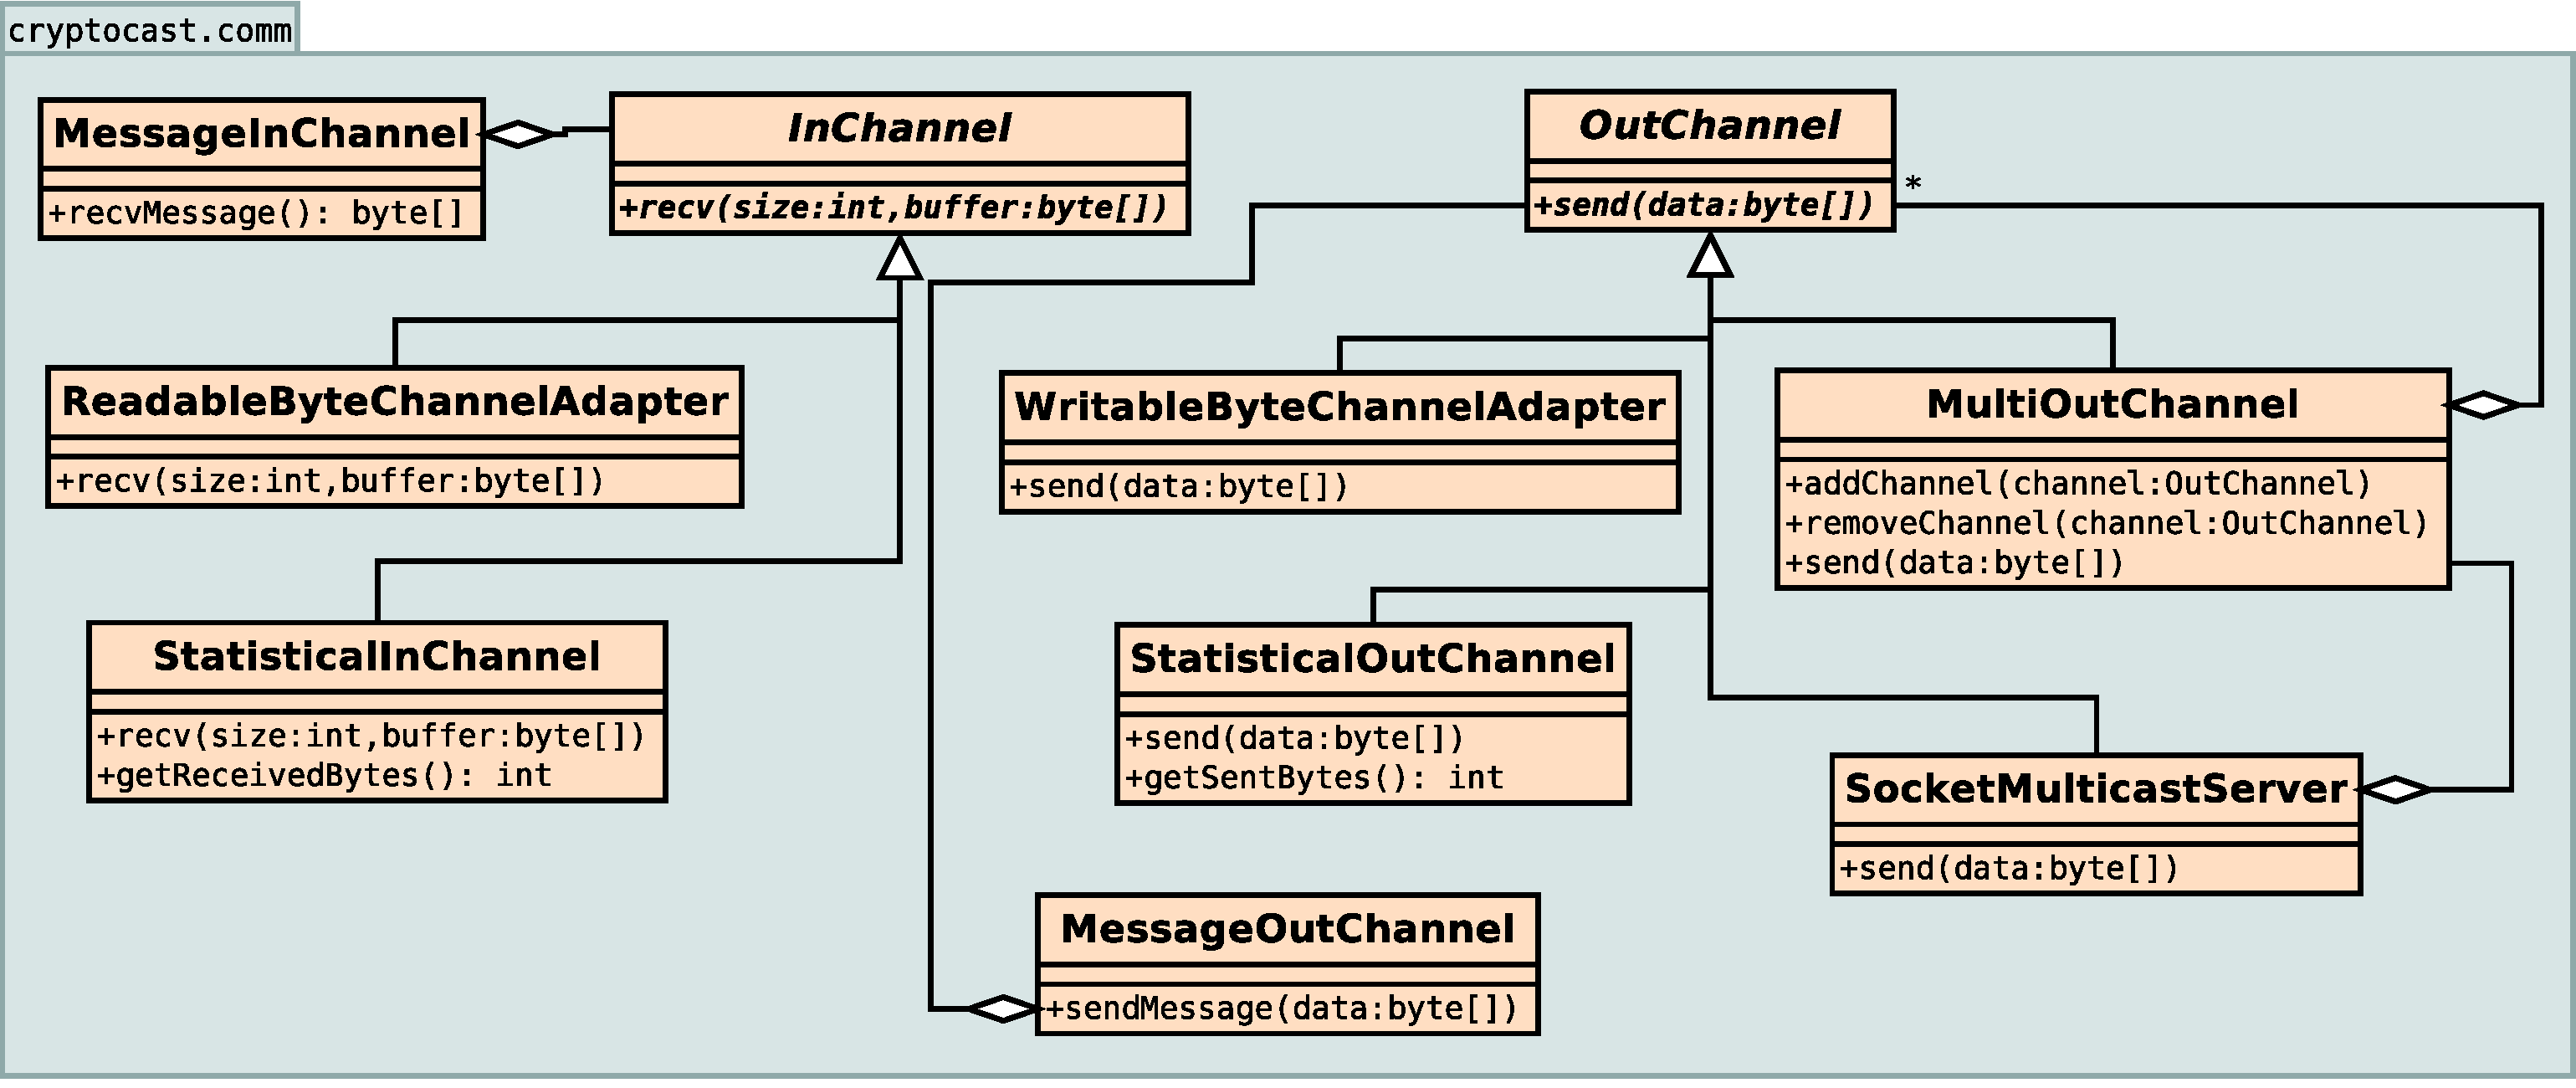
\includegraphics[width=450px]{class_diagrams/cryptocast_comm.pdf}
\end{minipage}

\subsubsection{Class \lstinline|WritableByteChannelAdapter|}
Adapter to use a \lstinline|WritableByteChannel| (for example, a file or socket instance) as
 an \lstinline|OutChannel|. \\
\noindent\begin{minipage}[t]{5cm}
\vspace{0.3em}
\hspace*{2em}
\begin{tikzpicture}
\umlclass[]{WritableByteChannelAdapter}{

}{
+ send(data : byte[])
}
\end{tikzpicture}
\vspace{0.3em}
\end{minipage}



\textbf{\sffamily Superclasses and Interfaces}
\begin{itemize}
\item \lstinline|cryptocast.comm.OutChannel|
\end{itemize}


\textbf{\sffamily Constructors}
\begin{itemize}
\item \lstinline|public| \lstinline|WritableByteChannelAdapter|\lstinline|(WritableByteChannel inner)|\\ \\[-0.6em]
Initializes the adapter
\begin{itemize}
\item \lstinline|inner|: The wrapped instance
\end{itemize}



\end{itemize}


\textbf{\sffamily Methods}
\begin{itemize}
\item \lstinline|public void| \lstinline|send|\lstinline|(byte[] data)|\\ \\[-0.6em]
Sends the given data.
\begin{itemize}
\item \lstinline|data|: the data to send
\end{itemize}



\end{itemize}

\subsubsection{Class \lstinline|StatisticalOutChannel|}
Wrapper around an \lstinline|OutChannel| that counts outgoing bytes. \\
\noindent\begin{minipage}[t]{5cm}
\vspace{0.3em}
\hspace*{2em}
\begin{tikzpicture}
\umlclass[]{StatisticalOutChannel}{

}{
+ send(data : byte[]) \\ + getSentBytes() : int
}
\end{tikzpicture}
\vspace{0.3em}
\end{minipage}



\textbf{\sffamily Superclasses and Interfaces}
\begin{itemize}
\item \lstinline|cryptocast.comm.OutChannel|
\end{itemize}


\textbf{\sffamily Constructors}
\begin{itemize}
\item \lstinline|public| \lstinline|StatisticalOutChannel|\lstinline|(OutChannel inner)|\\ \\[-0.6em]
Initializes the proxy
\begin{itemize}
\item \lstinline|inner|: the wrapped channel
\end{itemize}



\end{itemize}


\textbf{\sffamily Methods}
\begin{itemize}
\item \lstinline|public void| \lstinline|send|\lstinline|(byte[] data)|\\ \\[-0.6em]
Sends the given data.
\begin{itemize}
\item \lstinline|data|: the data to send
\end{itemize}



\item \lstinline|public int| \lstinline|getSentBytes|\lstinline|()|\\ \\[-0.6em]
\emph{Returns:} the number of sent bytes



\end{itemize}

\subsubsection{Class \lstinline|SocketMulticastServer|}
This class implements channel-based communication via TCP. \\
\noindent\begin{minipage}[t]{5cm}
\vspace{0.3em}
\hspace*{2em}
\begin{tikzpicture}
\umlclass[]{SocketMulticastServer}{

}{
+ send(data : byte[])
}
\end{tikzpicture}
\vspace{0.3em}
\end{minipage}



\textbf{\sffamily Superclasses and Interfaces}
\begin{itemize}
\item \lstinline|cryptocast.comm.OutChannel|
\end{itemize}


\textbf{\sffamily Constructors}
\begin{itemize}
\item \lstinline|public| \lstinline|SocketMulticastServer|\lstinline|(ServerSocket socket)|\\ \\[-0.6em]
Creates a multicast server which uses the given socket.
\begin{itemize}
\item \lstinline|socket|: server socket
\end{itemize}



\end{itemize}


\textbf{\sffamily Methods}
\begin{itemize}
\item \lstinline|public void| \lstinline|send|\lstinline|(byte[] data)|\\ \\[-0.6em]
Sends bytes via the channel.
\begin{itemize}
\item \lstinline|data|: the data to send
\end{itemize}



\end{itemize}

\subsubsection{Class \lstinline|MessageInChannel|}
Wraps a byte-based InChannel and allows to use it as a message-based
 channel. \\
\noindent\begin{minipage}[t]{5cm}
\vspace{0.3em}
\hspace*{2em}
\begin{tikzpicture}
\umlclass[]{MessageInChannel}{

}{
+ recvMessage() : byte[]
}
\end{tikzpicture}
\vspace{0.3em}
\end{minipage}




\textbf{\sffamily Constructors}
\begin{itemize}
\item \lstinline|public| \lstinline|MessageInChannel|\lstinline|(InChannel inner)|\\ \\[-0.6em]
Creates a MessageInChannel which wraps the given inner channel.
\begin{itemize}
\item \lstinline|inner|: the wrapped channel
\end{itemize}



\end{itemize}


\textbf{\sffamily Methods}
\begin{itemize}
\item \lstinline|public byte[]| \lstinline|recvMessage|\lstinline|()|\\ \\[-0.6em]
Receives a message via the channel.

\emph{Returns:} the received data

\end{itemize}

\subsubsection{Class \lstinline|MessageOutChannel|}
Wraps a byte-based OutChannel and allows to use it as a message-based
 channel. \\
\noindent\begin{minipage}[t]{5cm}
\vspace{0.3em}
\hspace*{2em}
\begin{tikzpicture}
\umlclass[]{MessageOutChannel}{

}{
+ sendMessage(data : byte[])
}
\end{tikzpicture}
\vspace{0.3em}
\end{minipage}




\textbf{\sffamily Constructors}
\begin{itemize}
\item \lstinline|public| \lstinline|MessageOutChannel|\lstinline|(OutChannel inner)|\\ \\[-0.6em]
Creates a new MessageOutChannel with the given OutChannel as inner channel.
\begin{itemize}
\item \lstinline|inner|: the OutChannel which will be wrapped
\end{itemize}



\end{itemize}


\textbf{\sffamily Methods}
\begin{itemize}
\item \lstinline|public void| \lstinline|sendMessage|\lstinline|(byte[] data)|\\ \\[-0.6em]
Sends the given message via the channel.
\begin{itemize}
\item \lstinline|data|: the data to send
\end{itemize}



\end{itemize}

\subsubsection{Class \lstinline|StatisticalInChannel|}
Wrapper around an \lstinline|InChannel| that counts incoming bytes \\
\noindent\begin{minipage}[t]{5cm}
\vspace{0.3em}
\hspace*{2em}
\begin{tikzpicture}
\umlclass[]{StatisticalInChannel}{

}{
+ recv(size : int, buffer : byte[]) \\ + getReceivedBytes() : int
}
\end{tikzpicture}
\vspace{0.3em}
\end{minipage}



\textbf{\sffamily Superclasses and Interfaces}
\begin{itemize}
\item \lstinline|cryptocast.comm.InChannel|
\end{itemize}


\textbf{\sffamily Constructors}
\begin{itemize}
\item \lstinline|public| \lstinline|StatisticalInChannel|\lstinline|(InChannel inner)|\\ \\[-0.6em]
Initializes the proxy
\begin{itemize}
\item \lstinline|inner|: the wrapped channel
\end{itemize}



\end{itemize}


\textbf{\sffamily Methods}
\begin{itemize}
\item \lstinline|public void| \lstinline|recv|\lstinline|(int size, byte[] buffer)|\\ \\[-0.6em]
Receives data.
\begin{itemize}
\item \lstinline|size|: maximum amount of bytes to read
\item \lstinline|buffer|: the target buffer
\end{itemize}



\item \lstinline|public int| \lstinline|getReceivedBytes|\lstinline|()|\\ \\[-0.6em]
\emph{Returns:} the number of received bytes



\end{itemize}

\subsubsection{Class \lstinline|ReadableByteChannelAdapter|}
Adapter to use a \lstinline|ReadableByteChannel| (for example, a file or socket instance) as an
 \lstinline|InChannel|. \\
\noindent\begin{minipage}[t]{5cm}
\vspace{0.3em}
\hspace*{2em}
\begin{tikzpicture}
\umlclass[]{ReadableByteChannelAdapter}{

}{
+ recv(size : int, buffer : byte[])
}
\end{tikzpicture}
\vspace{0.3em}
\end{minipage}



\textbf{\sffamily Superclasses and Interfaces}
\begin{itemize}
\item \lstinline|cryptocast.comm.InChannel|
\end{itemize}


\textbf{\sffamily Constructors}
\begin{itemize}
\item \lstinline|public| \lstinline|ReadableByteChannelAdapter|\lstinline|(ReadableByteChannel inner)|\\ \\[-0.6em]
Initializes the adapter
\begin{itemize}
\item \lstinline|inner|: The wrapped instance
\end{itemize}



\end{itemize}


\textbf{\sffamily Methods}
\begin{itemize}
\item \lstinline|public void| \lstinline|recv|\lstinline|(int size, byte[] buffer)|\\ \\[-0.6em]
Receives data.
\begin{itemize}
\item \lstinline|size|: maximum amount of bytes to read
\item \lstinline|buffer|: the target buffer
\end{itemize}



\end{itemize}

\subsubsection{Class \lstinline|MultiOutChannel|}
Multiplexes several \lstinline|OutChannel|s so that they can be used as a single
 destination. \\
\noindent\begin{minipage}[t]{5cm}
\vspace{0.3em}
\hspace*{2em}
\begin{tikzpicture}
\umlclass[]{MultiOutChannel}{

}{
+ addChannel(channel : OutChannel) \\ + removeChannel(channel : OutChannel) \\ + send(data : byte[])
}
\end{tikzpicture}
\vspace{0.3em}
\end{minipage}



\textbf{\sffamily Superclasses and Interfaces}
\begin{itemize}
\item \lstinline|cryptocast.comm.OutChannel|
\end{itemize}



\textbf{\sffamily Methods}
\begin{itemize}
\item \lstinline|public void| \lstinline|addChannel|\lstinline|(OutChannel channel)|\\ \\[-0.6em]
Adds the given channel to the list of receivers.
\begin{itemize}
\item \lstinline|channel|: the channel to add
\end{itemize}



\item \lstinline|public void| \lstinline|removeChannel|\lstinline|(OutChannel channel)|\\ \\[-0.6em]
Removes the given channel from the list of receivers.
\begin{itemize}
\item \lstinline|channel|: the channel to remove
\end{itemize}



\item \lstinline|public void| \lstinline|send|\lstinline|(byte[] data)|\\ \\[-0.6em]
Sends the given data.
\begin{itemize}
\item \lstinline|data|: the data to send
\end{itemize}



\end{itemize}

\subsubsection{Interface \lstinline|InChannel|}
A byte-based communication channel from which data can be received. \\
\noindent\begin{minipage}[t]{5cm}
\vspace{0.3em}
\hspace*{2em}
\begin{tikzpicture}
\umlclass[type=abstract]{InChannel}{

}{
\umlvirt{+ recv(size : int, buffer : byte[])}
}
\end{tikzpicture}
\vspace{0.3em}
\end{minipage}





\textbf{\sffamily Methods}
\begin{itemize}
\item \lstinline|public void| \lstinline|recv|\lstinline|(int size, byte[] buffer)|\\ \\[-0.6em]
Receives data.
\begin{itemize}
\item \lstinline|size|: maximum amount of bytes to read
\item \lstinline|buffer|: The target buffer
\end{itemize}



\end{itemize}

\subsubsection{Interface \lstinline|OutChannel|}
A byte-based communication channel where data can be sent to. \\
\noindent\begin{minipage}[t]{5cm}
\vspace{0.3em}
\hspace*{2em}
\begin{tikzpicture}
\umlclass[type=abstract]{OutChannel}{

}{
\umlvirt{+ send(data : byte[])}
}
\end{tikzpicture}
\vspace{0.3em}
\end{minipage}





\textbf{\sffamily Methods}
\begin{itemize}
\item \lstinline|public void| \lstinline|send|\lstinline|(byte[] data)|\\ \\[-0.6em]
Sends the given data.
\begin{itemize}
\item \lstinline|data|: the data to send
\end{itemize}



\end{itemize}


